% !TEX root = ../main.tex
\chapter{Implementation Details}
\label{chapter:DetailedDescriptions}\label{appendix}
We use python 3.10 on ubuntu 20.04. An overview of the used software and respective versions is shown in table \ref{tab:software_versions}. 

\begin{table}[H]
    \centering
    \begin{tabular}{|c|c|}
    \hline
    {} & Software Version \\
    \hline\hline
    Ubuntu & 20.04 \\
    \hline
    Python & 3.10 \\
    \hline
    PyTorch & 1.13\\
    \hline
    Numpy & 1.23.3 \\
    \hline
    MuJoCo & 2.1.2.14\\
    \hline
    Meta-World & 0.1.0\\
    \hline
    \end{tabular}
    \caption{Used software versions.}
    \label{tab:software_versions}
\end{table}

We use the planner, actor, and critic network implemented in PyTorch with an AdamW optimizer with learning rate 1e-4 and weight decay 1e-2. The 
critic has a linear head, which projects the $1 \times l$ results from the critic transformer to $1$ output for the whole sequence, where $l$ is the 
sequence length. \\

The hyperparameters of the models are depicted in table \ref{tab:model_parameters}. The dimensions in brackets hint how the total dimensions are 
computed. For example, the actor in Meta-World has 39 input dimensions from the observation space and a 1-dimensional input from the planner.

\begin{table}[H]
    \centering
    \begin{tabular}{|c|c|}
    \hline
    Hyperparameter & Value \\
    \hline\hline
    Model Dimension & 200 \\
    \hline
    Hidden Dimension & 200 \\
    \hline
    Attention Heads & 8\\
    \hline
    Layers & 5 \\
    \hline
    Sequence Length & 100\\
    \hline
    Actor Input Dimension& Meta-World: 40 (39 + 1), Language Conditioned: 45 (44 + 1)\\
    \hline
    Planner Input Dimension&Meta-World: 4, Language Conditioned: 7\\
    \hline
    Critic Input Dimension& Meta-World: 43 (39 + 4), Language Conditioned: 51 (44 + 7)\\
    \hline
    Actor Output Dimension& Meta-World: 4, Language Conditioned: 7\\
    \hline
    Planner Output Dimension & 1\\
    \hline
    Critic Output Dimension& 1\\
    \hline
    \end{tabular}
    \caption{Model Parameters.}
    \label{tab:model_parameters}
\end{table}


For training, we sample whole trajectories randomly from the replay buffer with batch size 16. The maximum size of the replay buffer is 50000 trajectories. 
We use at least 6000 trajectories or the whole replay buffer between two validation episodes in \ac{sopomdp}s and at least 1000 trajectories or the whole 
replay buffer in \ac{mdp}s. We add 10 training episodes at once after each validation. To prevent early overfitting of the critic given limited data, 
we only train the critic until the train loss is 1e-5.
\\

In inference time, we use different optimizer settings for \ac{sopomdp}s and \ac{mdp}s, which are depicted in table \ref{tab:inference_parameters}. 
In environments with no provided expert trajectories, we used an inference time learning rate of 1e-6 until we found three successful trajectories. 
After that, we used a learning rate of 1e-5, which resulted in quicker convergence. 


\begin{table}[H]
    \centering
    \begin{tabular}{|c|c|}
    \hline
    {} & \textbf{\ac{sopomdp}} \\
    \hline\hline
    Optimizer & AdamW \\
    \hline
    Learning Rate & 1e-6 \\
    \hline
    Optimization Steps & 100 per trajectory\\
    \hline\hline
    {} & \textbf{\ac{mdp}}  \\
    \hline\hline
    Optimizer & AdamW \\
    \hline
    Learning Rate Exploration / Finetuning & 1e-6 \\
    \hline
    Learning Rate Exploitation & 1e-5 \\
    \hline
    Optimization Steps & 3 per step\\
    \hline
    Explore Until & 3 trajectories found\\
    \hline
    \end{tabular}
    \caption{Used software versions.}
    \label{tab:inference_parameters}
\end{table}

We sample 10 trajectories in parallel for training inference and 15 trajectories in parallel twice per data point for evaluation. During inference time 
optimization, we only optimize trajectories, for which the critic value is smaller then 1. We clip the actions to stay within the boundaries of the environments.\\


\chapter{Meta World}
\label{chapter:MetaWorld}
\begin{figure}[h]
    \centering
    \begin{subfigure}[b]{1\linewidth}
    \includegraphics[width=0.18\linewidth]{images/meta-world/pick_place/cropped/0_cropped.png}
    \includegraphics[width=0.18\linewidth]{images/meta-world/pick_place/cropped/1_cropped.png}
    \includegraphics[width=0.18\linewidth]{images/meta-world/pick_place/cropped/2_cropped.png}
    \includegraphics[width=0.18\linewidth]{images/meta-world/pick_place/cropped/3_cropped.png}
    \includegraphics[width=0.18\linewidth]{images/meta-world/pick_place/cropped/4_cropped.png}
    \caption{Expert demonstration of the Pick and Place environment.}
    \end{subfigure}
    \begin{subfigure}[b]{1\linewidth}
        \includegraphics[width=0.18\linewidth]{images/meta-world/push/cropped/0_cropped.png}
        \includegraphics[width=0.18\linewidth]{images/meta-world/push/cropped/1_cropped.png}
        \includegraphics[width=0.18\linewidth]{images/meta-world/push/cropped/2_cropped.png}
        \includegraphics[width=0.18\linewidth]{images/meta-world/push/cropped/3_cropped.png}
        \includegraphics[width=0.18\linewidth]{images/meta-world/push/cropped/4_cropped.png}
        \caption{Expert demonstration of the Push environment.}
    \end{subfigure}
    \begin{subfigure}[b]{1\linewidth}
        \includegraphics[width=0.18\linewidth]{images/meta-world/reach/cropped/0_cropped.png}
        \includegraphics[width=0.18\linewidth]{images/meta-world/reach/cropped/1_cropped.png}
        \includegraphics[width=0.18\linewidth]{images/meta-world/reach/cropped/2_cropped.png}
        \includegraphics[width=0.18\linewidth]{images/meta-world/reach/cropped/3_cropped.png}
        \includegraphics[width=0.18\linewidth]{images/meta-world/reach/cropped/4_cropped.png}
        \caption{Expert demonstration of the Reach environment.}
    \end{subfigure}
    \begin{subfigure}[b]{1\linewidth}
        \includegraphics[width=0.18\linewidth]{images/meta-world/window_open/cropped/0_cropped.png}
        \includegraphics[width=0.18\linewidth]{images/meta-world/window_open/cropped/1_cropped.png}
        \includegraphics[width=0.18\linewidth]{images/meta-world/window_open/cropped/2_cropped.png}
        \includegraphics[width=0.18\linewidth]{images/meta-world/window_open/cropped/3_cropped.png}
        \includegraphics[width=0.18\linewidth]{images/meta-world/window_open/cropped/4_cropped.png}
        \caption{Expert demonstration of the Window Open environment.}
    \end{subfigure}
    \begin{subfigure}[b]{1\linewidth}
        \includegraphics[width=0.18\linewidth]{images/meta-world/drawer_close/cropped/0_cropped.png}
        \includegraphics[width=0.18\linewidth]{images/meta-world/drawer_close/cropped/1_cropped.png}
        \includegraphics[width=0.18\linewidth]{images/meta-world/drawer_close/cropped/2_cropped.png}
        \includegraphics[width=0.18\linewidth]{images/meta-world/drawer_close/cropped/3_cropped.png}
        \includegraphics[width=0.18\linewidth]{images/meta-world/drawer_close/cropped/4_cropped.png}
        \caption{Expert demonstration of the Drawer Close environment.}
    \end{subfigure}
    \caption{Meta-World tasks with expert demonstrations.}
    \label{fig:meta-world}
\end{figure}
  


The Meta-World benchmark suite, consisting of 50 challenging robotic manipulation tasks designed to assess the capabilities of reinforcement learning (RL) algorithms, 
has been introduced by Yu \etAl \cite{yu2019meta}. Meta-World is widely utilized in meta-\ac{rl} and \ac{rl} tasks.

One of the key advantages of Meta-World is the well-defined success criteria for the tasks, enabling the definition of sparse rewards in a natural way. 
In this thesis, we select five environments from the ML10 suite, namely "Pick and Place", "Window Open", "Drawer Close", "Push", and "Reach", which provide diverse and varying levels of 
difficulty. The corresponding environments, along with expert demonstrations, are depicted in figure \ref{fig:meta-world}. In "Reach," "Pick and Place," and "Push," the position of the goal 
and the puck are randomly generated for each instance of the environment, whereas in "Window Open," the window's position changes, and in "Drawer Close," the drawer's position is variable.

The observation space consists of 39 dimensions, including a three-dimensional representation of the goal, while the action space is four-dimensional. For our experiments, 
we employ the goal-observable V2 environments. Meta-World uses the MuJoCo simulation environment \cite{todorov2012mujoco}, which is an efficient physics-based 
simulator capable of simulating object interactions such as puck grasping or window sliding.

\chapter{Additional Plots}
\label{chapter:additional_plots}

\begin{figure}[htbp]
    \centering
    \begin{subfigure}[b]{0.45\textwidth}
      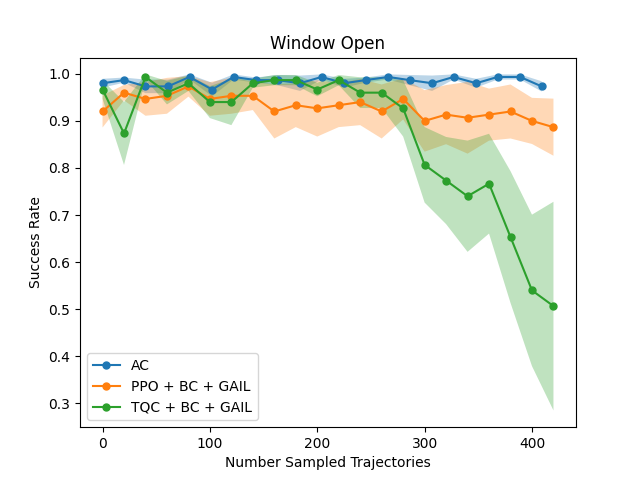
\includegraphics[width=\textwidth]{images/15_400/Window Open.png}
      \caption{Window Open environment.}
    \end{subfigure}
    \hfill
    \begin{subfigure}[b]{0.45\textwidth}
      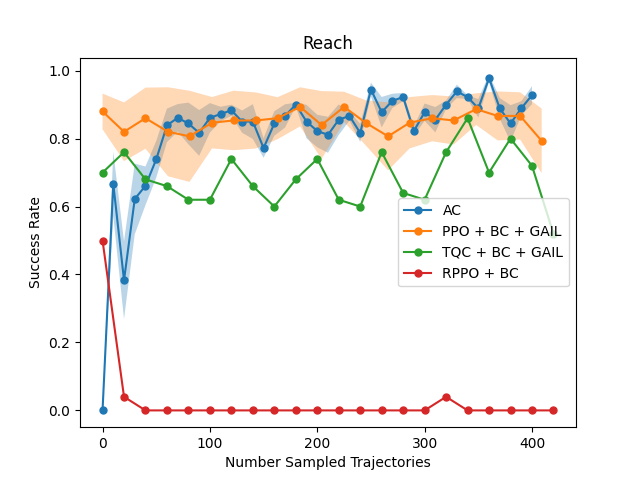
\includegraphics[width=\textwidth]{images/15_400/Reach.png}
      \caption{Reach environment.}
    \end{subfigure}
    \medskip
    \begin{subfigure}[b]{0.45\textwidth}
      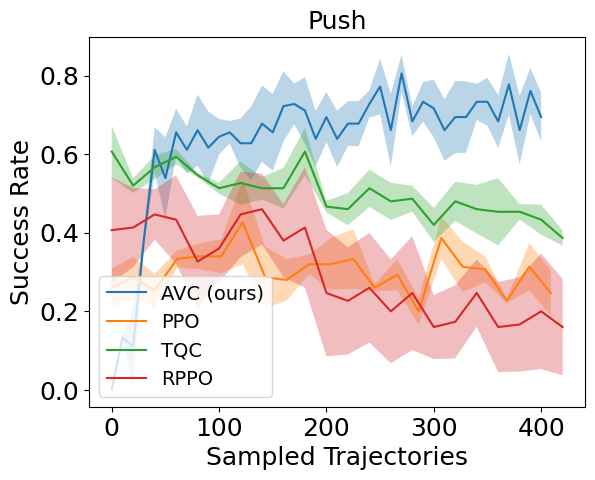
\includegraphics[width=\textwidth]{images/15_400/Push.png}
      \caption{Push environment.}
    \end{subfigure}
    \hfill
    \begin{subfigure}[b]{0.45\textwidth}
      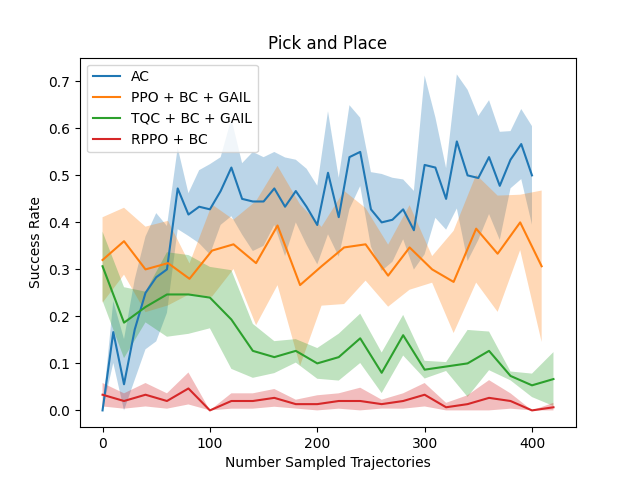
\includegraphics[width=\textwidth]{images/15_400/Pick and Place.png}
      \caption{Pick and Place environment.}
    \end{subfigure}
    \caption{All learners were pretrained using behavioral cloning with the given 15 expert demonstrations. 
    The x-axis shows the number of sampled environment episodes, each with 100 steps.  One initial observation and a sparse reward signal at the end of each episode was provided. 
    The shaded area indicates the standard deviations from four runs per experiment.}
\end{figure}

\begin{figure}[htbp]
  \centering
  \begin{subfigure}[b]{0.45\textwidth}
    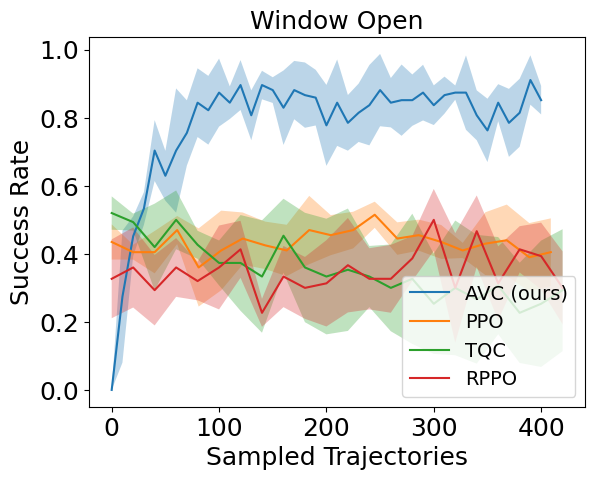
\includegraphics[width=\textwidth]{images/4_400/Window Open.png}
    \caption{Window Open environment.}
  \end{subfigure}
  \hfill
  \begin{subfigure}[b]{0.45\textwidth}
    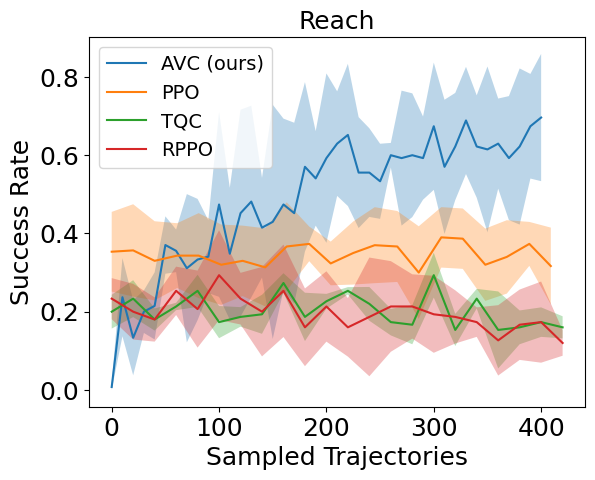
\includegraphics[width=\textwidth]{images/4_400/Reach.png}
    \caption{Reach environment.}
  \end{subfigure}
  \medskip
  \begin{subfigure}[b]{0.45\textwidth}
    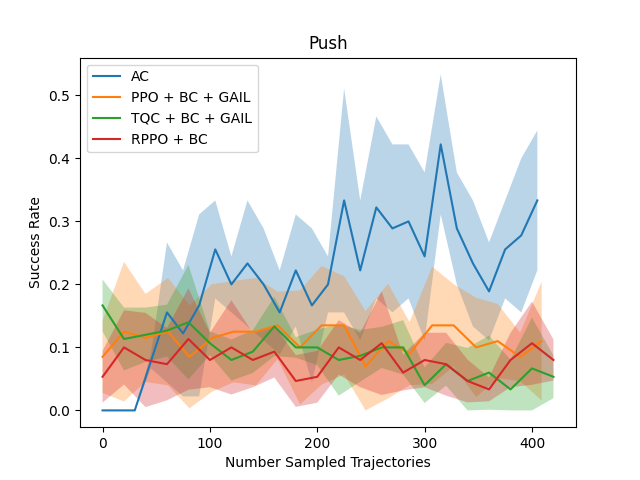
\includegraphics[width=\textwidth]{images/4_400/Push.png}
    \caption{Push environment.}
  \end{subfigure}
  \hfill
  \begin{subfigure}[b]{0.45\textwidth}
    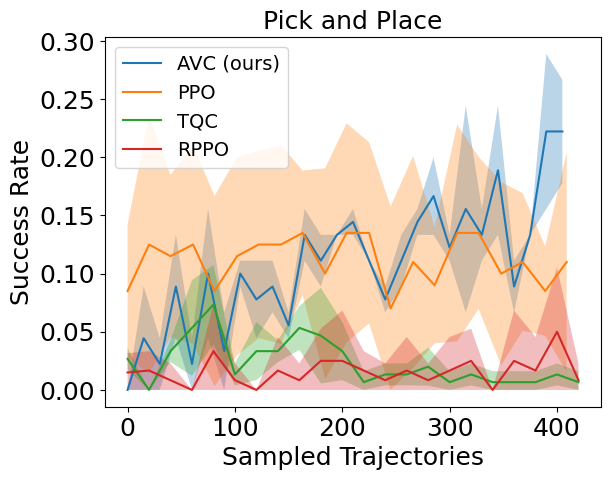
\includegraphics[width=\textwidth]{images/4_400/Pick and Place.png}
    \caption{Pick and Place environment.}
  \end{subfigure}
  \caption{All learners were pretrained using behavioral cloning with the given 4 expert demonstrations. 
  The x-axis shows the number of sampled environment episodes, each with 100 steps.  One initial observation and a sparse reward signal at the end of each episode was provided. 
  The shaded area indicates the standard deviations from four runs per experiment.}
\end{figure}

\chapter{Generative Adversarial Imitation Learning}
\label{app:GAIL}
For \ac{il}, Generative Adversarial Imitation Learning (GAIL) 
\cite{ho2016generative} presents a key paradigm to make efficient use of expert demonstrations given access to the \ac{mdp}. 
The main idea of \ac{gail} is to disambiguate the reward signal 
by ensuring every policy except the expert policy has a lower expected reward under our inverse reward function, given the expert 
demonstrations.\\ 
First, 
maximum causal entropy IRL \cite{10.5555/3104322.3104481} is a method to regularize policies found from \ac{irl}. The idea is to choose the reward function, for 
which the optimal policy has the highest entropy with respect to the action distribution. This allows us to choose a policy that is "no more committed to any 
particular path" \cite[p.2]{10.5555/3104322.3104481}, then necessary. Formally the objective is written as:
\begin{equation*}
    \label{proto_inf_ler_app}
    \underset{r_{\text{inv}} \in \mathcal{R}}{\text{minimize}} \left( \max_{\pi \in \Pi} \left( - \text{H}(\pi) + \mathbb{E}_{\pi}[r_{\text{inv}}(s, a)] \right) - \mathbb{E}_{\pi_{r'}^*}[r_{\text{inv}}(s,a)] \right),
\end{equation*}
with the discounted expected reward
\begin{equation*}
    \mathbb{E}_{\pi}[r(s, a)] =
    \mathbb{E}_{(s,a,t) \propto \pi}[\gamma^t r(s,a)] = 
    \mathbb{E}_{\tau \sim p(\tau | \pi)} \left[ \sum_{t=0}^\infty \gamma^t r_t \right]
\end{equation*}
and the discounted causal entropy as defined by Bloem \etAl \cite{InfCausalEnt}:
\begin{equation*}
    \mathbb{H}(\pi) = \mathbb{E}_{s_0, a_0} \left(\text{H}_{\pi}(a_{0...\infty}, s_{0,...\infty})\right) = \mathbb{E}_{\pi}\left[\sum_{t=0}^\infty -\gamma^t log \pi(a_t|s_t)\right].
\end{equation*}
Here $\pi_{r'}^*$ denotes the expert policy, which indicates the expert policy is assumed to maximize a true 
reward function ${r'}$. From now, we will refer to the expert policy as $\pi_{\text{E}}$, as it is more in line with the common choice found in 
literature. Furthermore, we used the reward in equation  \ref{proto_inf_ler_app}, as it is in line with our notation for \ac{rl}. In the paper, 
the authors minimize a cost function $c$, instead of maximizing a reward function $r$. The choice does not make a profound 
mathematical difference, but it gives a more natural way to interpret the inverse objective. $c=0$ can be naturally defined as the optimal cost value, while a reward function has 
no natural upper bound. For this practical reason, we will make use of $c$ instead of $r$ for the rest of this section. As $c \propto -r$, the minimization in 
\ref{proto_inf_ler_app} becomes a maximization and vice versa:
\begin{equation}
    \label{proto_inf_ler_c_app}
    \pi_{\text{inv}}^* = \underset{c_{\text{inv}} \in \mathcal{C}}{\text{max}} \left( \min_{\pi \in \Pi} \left(- \text{H}(\pi) + \mathbb{E}_{\pi}[c_{\text{inv}}(s, a)] \right) - \mathbb{E}_{\pi_{\text{E}}}[c_{\text{inv}}(s,a)] \right).
\end{equation}
The key insight is, that this optimization problem can be uniquely identified with an occupancy measure distance between the expert policy and the 
induced policy. Intuitively, an occupancy measure is a measure for how likely a policy visits a state action pair given the \ac{mdp}. If two policies visit the same 
states and choose the same actions, they are similar to each other.\\
Formally the occupancy measure for states and actions is defined by: 
\begin{equation*}
    \rho_{\pi}:\mathcal{S} \times \mathcal{A} \rightarrow \mathbb{R} = \pi(a|s)\sum_{t=0}^\infty \gamma^tP(s_t=s|\pi).
\end{equation*}
With this, the discounted expected reward can be written as:
\begin{equation}
    \mathbb{E}_\pi[c(s,a)] = \sum_{s,a} \rho_\pi(s,a) c(s,a)
\end{equation}
and equation \ref{proto_inf_ler_c_app} can be written as:
\begin{equation}
    \label{occ_meas_obj_app}
    \pi_{\text{inv}}^* = \max_{c_{\text{inv}} \in \mathcal{C}} \left( \min_{\rho_\pi \propto \pi \in \Pi} \left(- \bar{\text{H}}(\rho_\pi) + \sum_{s,a} \rho_\pi(s,a) c(s,a) \right) - \sum_{s,a} \rho_{\text{E}}(s,a) c(s,a) \right).
\end{equation}

It is then shown that a policy is uniquely identified with its occupancy measure $\rho_{\pi} \propto \pi$. With this in mind, we rewrite equation \ref{proto_inf_ler_c_app} as a constrained satisfaction problem:
\begin{equation}
    \label{const_sat_gail_app}
    \pi_{\text{inv}}^* = \min_{\pi \propto \rho_{\pi}} - \bar{\text{H}}(\rho_{\pi})\quad \text{subject to }\quad \rho_{\pi}(s,a) = \rho_{\text{E}}(s,a) \quad \forall s \in \mathcal{S}, \forall a \in \mathcal{A},
\end{equation}
where $\bar{\text{H}}$ is the the discounted causal entropy $\text{H}$ defined on occupancy measures of policies, rather then action distributions. In this sense, equation \ref{proto_inf_ler_c_app} is the dual problem of equation \ref{const_sat_gail_app}. 
This optimization is intractable, as we get as many constraints, as we have action state pairs in our \ac{mdp}. Moreover, in practice we only have a small sample size, which would mean setting 
the occupancy measure for all unvisited state action pairs to zero. This is obviously not the intended optimum. Instead, the objective \ref{const_sat_gail_app} is relaxed:
\begin{equation}
    \label{dist_opt_app}
    \pi_{\text{inv}}^* = \min_{\pi} d_{\psi}(\rho_{\pi_{\text{E}}}, \rho_{\pi}) - \text{H}(\pi)
\end{equation}
such that $d_{\psi}$ becomes small, when $\pi_{\text{E}}$ and $\rho_{\pi}$ become similar. To do this, we can introduce an additional regularizor $\psi$ to equation \ref{occ_meas_obj_app}:

\begin{equation*}
    \pi_{\text{inv}}^* = \max_{c_{\text{inv}} \in \mathcal{C}} \left(-\psi(c) \ \min_{\rho_\pi \propto \pi \in \Pi} \left(- \bar{\text{H}}(\rho_\pi) + \sum_{s,a} \rho_\pi(s,a) c(s,a) \right) - \sum_{s,a} \rho_{\text{E}}(s,a) c(s,a) \right)
\end{equation*}
\begin{equation*}
    = \min_{\rho_\pi \propto \pi \in \Pi}- \bar{\text{H}}(\rho_\pi) + \max_{c_{\text{inv}} + \in \mathcal{C}} -\psi(c) \sum_{s,a} \left( \rho_\pi(s,a) - \rho_{\text{E}}(s,a)\right) c(s,a)
\end{equation*}
\begin{equation}
    \label{proto_inf_ler_c_reg_app}
    = \min_{\rho_\pi \propto \pi \in \Pi}- \bar{\text{H}}(\rho_\pi) + \psi^*(\rho_\pi(s,a) - \rho_{\text{E}}(s,a)),
\end{equation}
where $\psi^*$ is the complex conjugate of $\psi$. With this, we can identify $d_{\psi} = \psi^*$.\\

What is left now is to find a $\psi$ s.t. minimizing \ref{dist_opt_app} ensures $\rho_{\pi} \sim \rho_{\text{E}}$. The authors propose $\psi_{\text{GA}}$, 
which complex conjugate $\psi^*_{\text{GA}}$ is: 
\begin{equation}
    \psi^*_{\text{GA}} = \max_{D\in(0,1)^{\mathcal{S} \times \mathcal{A}}} \mathbb{E}_{\pi}\left[ \text{log}(D(s,a))\right] + \mathbb{E}_{\pi_{\text{E}}}\left[ \text{log}(1 - D(s,a))\right],
\end{equation}
with discriminator $D$. In this formulation, the objective \ref{proto_inf_ler_c_reg_app} minimzes the Jensen Shannon divergence ($D_{JS}$) between $\rho_\pi$ and $\rho_{\text{E}}$. If we treat the entropy constraint as a regularization with 
parameter $\lambda$, the \ac{gail} objective can be written as:
\begin{equation}
    J(\rho_{\pi_{\theta}}, D_{\omega}) = - \lambda  \bar{\text{H}}(\rho_{\pi_{\theta}} ) + \mathbb{E}_{\pi_{\theta}}\left[ \text{log}(D_{\omega}(s,a))\right] + \mathbb{E}_{\pi_{\text{E}}}\left[ \text{log}(1 - D_{\omega}(s,a))\right],
\end{equation}
where $\omega$ and $\theta$ denote the parametrization of the discriminator $D$ and the policy $\pi$. Identifying the discounted reward as $Q = \mathbb{E}_{\pi}(r_t) = \mathbb{E}_{\pi}\left[-\text{log}(D_{\omega}(s,a))\right]$ and using the policy 
gradient theorem, we get the policy update rule:
\begin{equation}
    \label{GAIL_update_policy_app}
    \nabla_{\theta} J(\rho_{\pi_{\theta}}, D_{\omega}) = \mathbb{E}_{\tau \propto \pi}\left[ \nabla_{\theta}\text{log}\pi_{\theta}(a|s) Q(s,a) -\lambda \nabla_{\theta}\bar{\text{H}}(\rho_{\pi_{\theta}} )  \right]
\end{equation}
and the discrimnator update rule as:
\begin{equation}
    \label{eq_GAIL_disc_app}
    \nabla_{\omega} J(\rho_{\pi_{\theta}}, D_{\omega}) = \mathbb{E}_{\tau \propto \pi} [\nabla_w \mathrm{log}(D_w(s,a))] + {E}_{\tau_E} [\nabla_w \mathrm{log}(1 - D_w(s,a))].
\end{equation}
Note, because cost $c$ instead of reward $r$ is used in equation \ref{GAIL_update_policy_app} gradient descent is used, as the cost is minimized and in equation \ref{eq_GAIL_disc_app} 
gradient ascent is used, as we want to maximize the discriminative power of $D$. The algorithm is summarized in algorithm \ref{GAIL_Algo_app}.\\
\begin{algorithm}
    \caption{Generative Adversarial Imitation Learning}
    \label{GAIL_Algo_app}
    Require expert trajectories $\tau_E \sim \pi_E$, initial policy and discriminator parameters $\theta_0$, $w_0$\\
    \For{$i = 0, 1, 2, \dots$}{
        Sample trajectories $\tau_i \sim \pi_{\theta_i}$\\
        Update the discriminator parameters from $w_i$ to $w_{i+1}$ with the gradient\\
            \begin{equation}
            \hat{\mathbb{E}}_{\tau_i} [\nabla_w \log D_w(s, a)] + \hat{\mathbb{E}}_{\tau_E} [\nabla_w \mathrm{log}(1 - D_w(s, a))]
            \end{equation}
        Take a policy step from $\theta_i$ to $\theta_{i+1}$, using the \ac{trpo} rule with cost function $\log D_{w_{i+1}}(s, a)$.\\
        Specifically, take a KL-constrained natural gradient step with
        \begin{equation}
        \hat{\mathbb{E}}_{\tau_i} [\nabla\theta \log \pi_\theta(a|s)Q(s, a)] - \lambda \nabla_\theta H(\pi_\theta),
        \end{equation}
        where $Q(\bar{s}, \bar{a}) = \hat{\mathbb{E}}_{\tau_i} [\log D{w_{i+1}}(s, a) | s_0 = \bar{s}, a_0 = \bar{a}]$
    }
\end{algorithm}
Tian Xu \etAl proved that if a policy $\pi$ minimizes the $\text{D}_{JS}$ distance 
between occupancy measures of $\rho_{\pi^*}$ and $\rho_{\pi}$, the generalization error $V_{\pi^*} - V_{\pi_{\text{imitation}}}$ is bound by 
$V^{{\pi^*}} - V^{\pi} \leq \mathcal{O}\left(\frac{1}{\sqrt{1-\gamma}}\right)$, while the generalization error of behavioral cloning is bound by 
$V^{{\pi^*}} - V^{\pi} \leq \mathcal{O}\left(\frac{1}{\sqrt{1-\gamma^2}}\right)$ \cite{NEURIPS2020_b5c01503} . This explains better performance for\ac{gail} in long horizon tasks, which has 
been empirically demonstrated. Overall, \ac{gail} is a state-of-the-art imitation learning algorithm which is able to learn complex behavior with limited expert demonstrations. It shows outstanding 
asymptotical performance with respect to the amount of expert demonstrations but requires a high number of environment interactions to train the discriminator and actor as stated by the authors. 

\chapter{Language-Conditioned Imitation Learning for Robot Manipulation Tasks}
\label{LCILRM}
Simon Stepputtis \etAl \cite{stepputtis2020languageconditioned} propose a benchmark for natural language conditioned robot manipulation tasks. \\
The benchmark consists of a 7 dof simulated robot arm with a 
tabletop setup using CoppeliaSim, which allows for accurate dynamics simulations at an update rate of 20 Hz. 
An \ac{il} dataset consisting of 44 100 tasks is provieded, where 4000 tasks are used for 
evaluation and 100 tasks are used for testing.\\

The task consists of picking up objects and pouring their content into other objects. A sentense in natural language describes the task and the object. 
For example "Pick up the red cup". Additionally, an rgb image of the scene is provided. An overview over 
all possible objects and an example task can be found in figure \ref{lang_imi_expl}. 
There is only one observation per trajectory, so the setting is the single observation \ac{pomdp}.  \\


Simon Stepputtis \etAl \cite{stepputtis2020languageconditioned} also propose a method to solve the benchmark. 
The proposed method involves using a neural network to map natural language instructions to 
corresponding robot actions. The experimental results demonstrate the effectiveness of their approach in inferring and executing trajectories for robot manipulation 
tasks when language instructions are given. \\

In more detail, a policy $\pi(v,I)$ is learned to imitate expert behavior in a set of demonstrations $D = \{d_0,...,d_m\}$, each containing a trajectory 
$R \in R^{T \times N}$ over $T$ time steps and with $N$ control variables, an rgb image $I \in \mathcal{R}^{569 \times 320 \times 3}$ of the agent's surroundings, 
and a task description $v \in \mathcal{R}^{15 \times 50}$ from natural language. The proposed method takes the image $I$ and task description $v$ 
to create a task embedding $e$ using GloVe embeddings and a pretrained image recognition model in the semantic model, 
which is subsequently used in the control model to generate robot actions at each time step in a closed-loop 
fashion using a GRU to keep track of the former history. In addition to the hidden state of the GRU, 
the task embedding $e$ is used in every time step, as we know, that the task does not change. A schematic overview can be seen in figure \ref{language_imitation}. \\

\begin{figure}[htbp]
    \centering
    \includegraphics[width=\textwidth]{images/Language_Conditioned/System.pdf}
    \caption{Overview of the general system architecture. (Left) Details of the controller model, which
    synthesises robot control signals . (Right) details of the semantic model, which extracts critical
    information about the task from both perceptual input and language commands. Dark-blue boxes
    indicate pre-trained components of the model. The figure is taken from \cite{stepputtis2020languageconditioned}.}
    \label{language_imitation}
\end{figure}

The authors find that their model can perform $98 \%$ of pick tasks, $85 \%$ of pour tasks and $84 \%$ combined 
tasks, which greatly outperforms a baseline using an end-to-end RNN model with $58\%$ success rate for picking and $0 \%$ success rate for pouring.

\begin{figure}[htbp]
    \centering
    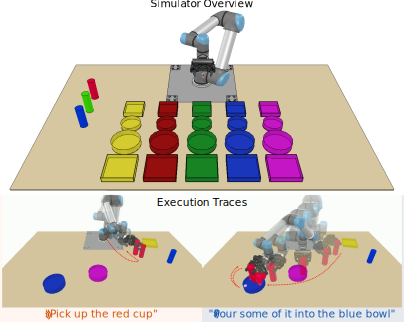
\includegraphics[width=0.4\textwidth]{images/Language_Conditioned/simulator.pdf}
    \caption{Overview of a task. (top) All possible objects and colors. (left) Example trajectory to "pick up the red cup" following the natural language description. 
    (right) Example trajectory to "pour some of it into the blue bowl". The figure is taken from \cite{stepputtis2020languageconditioned}.}
    \label{lang_imi_expl}
\end{figure}
